\section{Mechanism walkthrough}
\label{sec:mech}
This section follows the machine from the handwheel to the section ribbon, naming every part (Fig.~\ref{fig:concept}, numbered 1--20; Fig.~\ref{fig:section}, cut at $y=0$) and giving the governing relation for each stage with the numbers used in the design. Throughout, $x$ is the feed axis (specimen~$\rightarrow$~blade), $y$ runs along the blade edge, $z$ is up, and the pivot axis is the $y$-parallel line through $P=(0,0,95)$\,mm.

\begin{figure}[!htbp]\centering
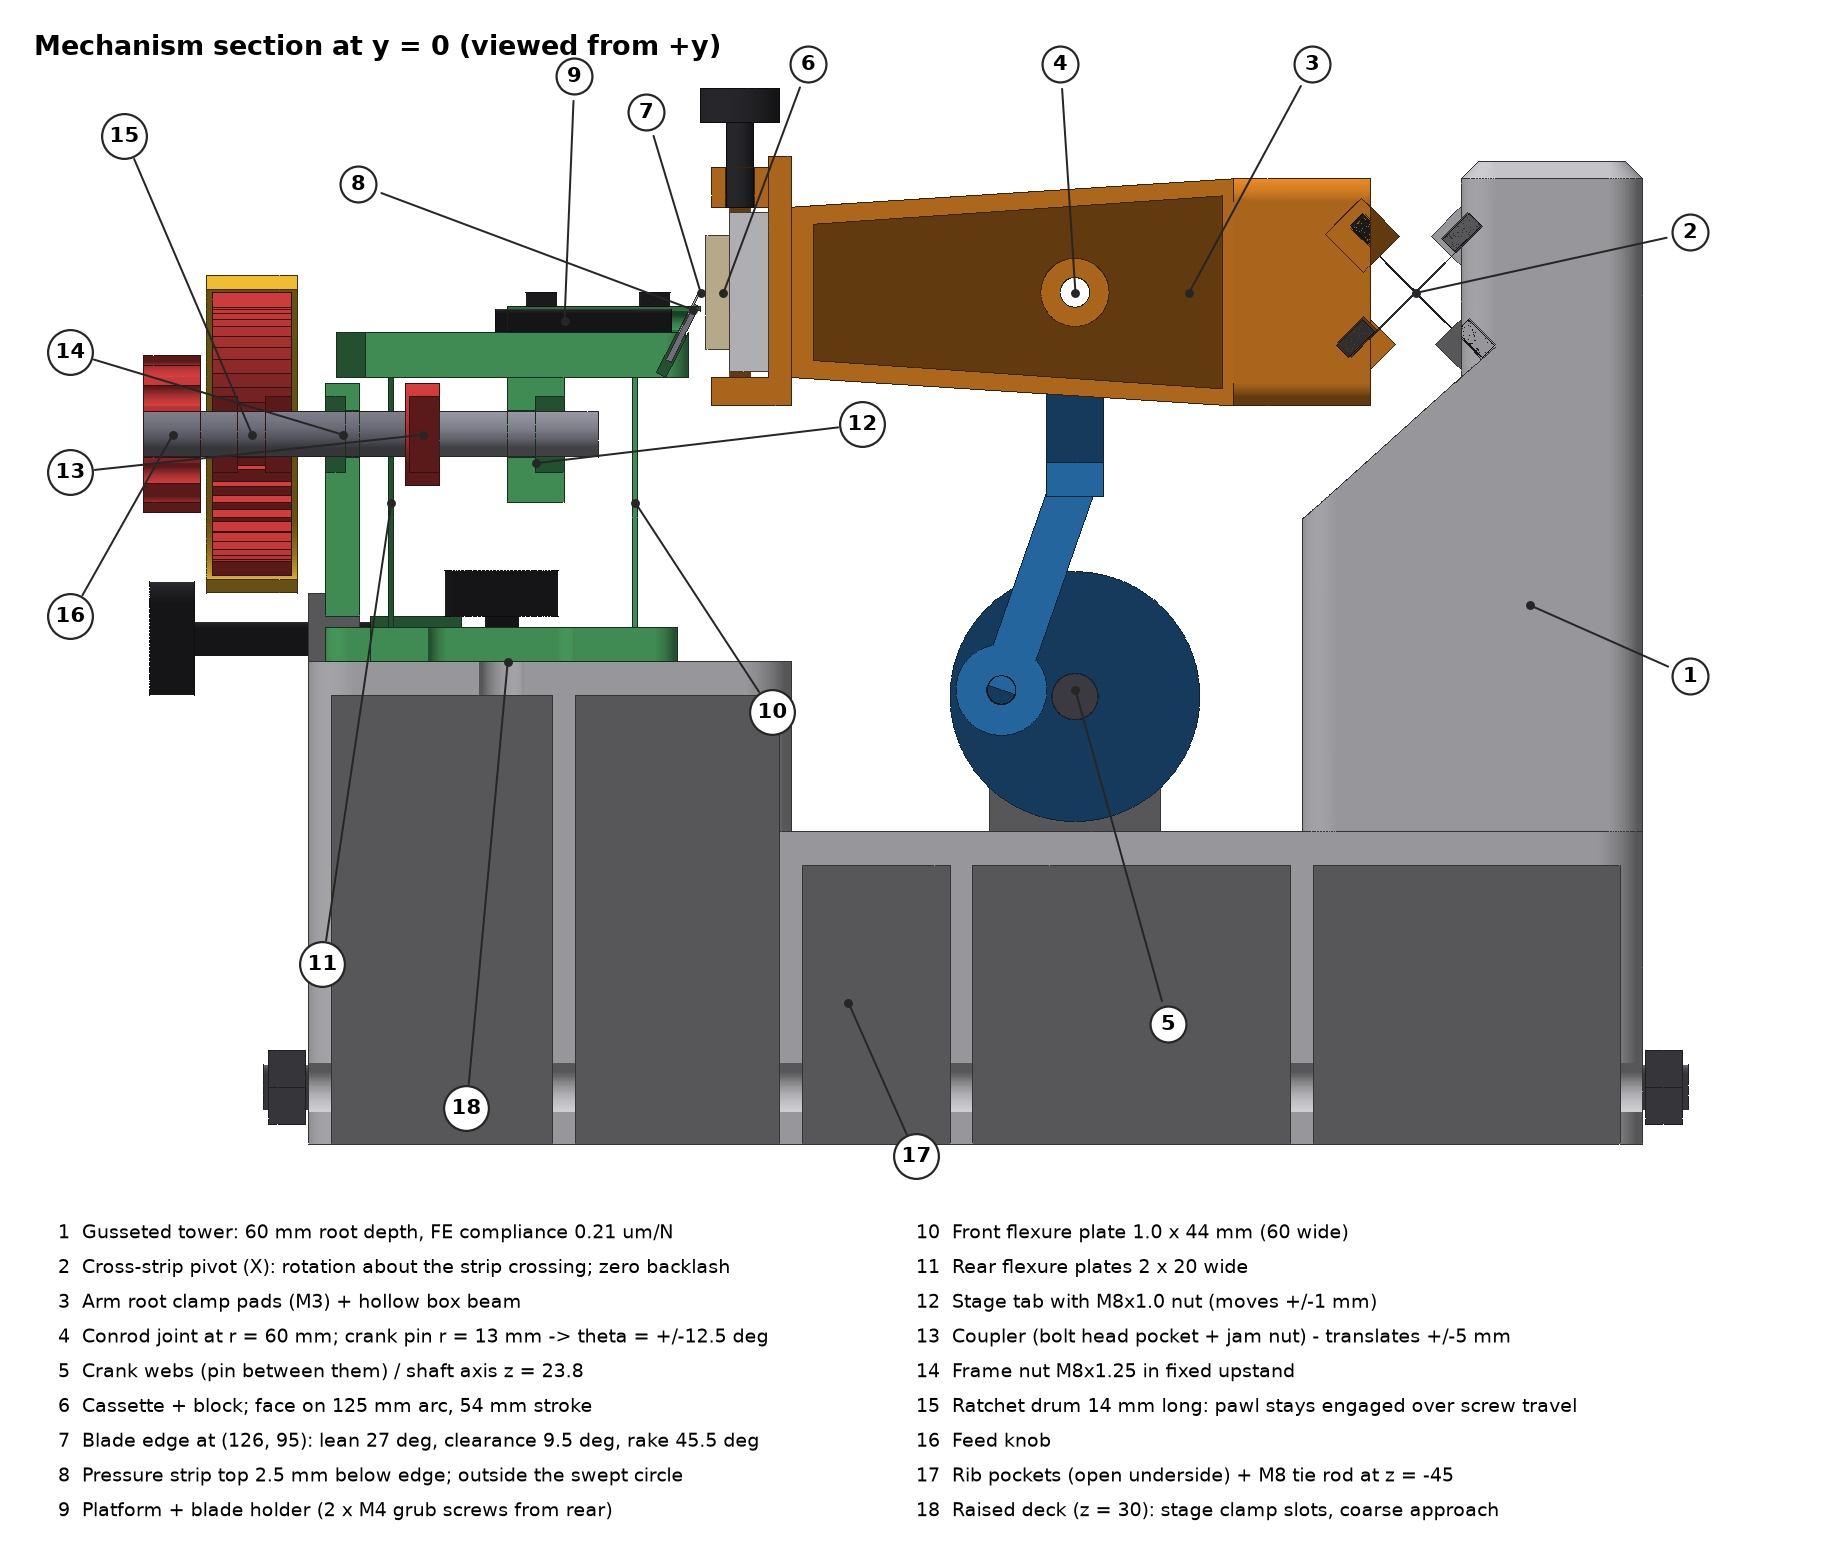
\includegraphics[width=\linewidth]{fig7_section_callouts.png}
\caption{Section through the mid-plane $y=0$, viewed from $+y$ (handwheel removed). The metrology loop runs from the blade edge (7) through the holder and platform (9), the flexure plates (10, 11), the stage nut tab (12), the differential screw and coupler (13), the frame nut (14), the deck and base (17, 18), the tower (1), the cross-strip pivot (2) and the arm (3) to the block face (6). The drive (crank webs (5), connecting rod (4)) hangs below the arm and is outside the loop.}
\label{fig:section}
\end{figure}

\FloatBarrier
\subsection{Drive train: handwheel to arm}
The handwheel (19; \SI{110}{\milli\metre}, five spokes, offset handle) turns a built-up crankshaft (18): two \SI{8}{\milli\metre} steel shaft stubs run in two 608 bearings in printed pillow blocks at $y=\pm50$\,mm, and are grub-screwed into two printed crank webs (\SI{44}{\milli\metre} diameter) that carry a \SI{5}{\milli\metre} crank pin at radius $r=\SI{13}{\milli\metre}$. The connecting rod (17) is a fork: its lower eye runs on the pin \emph{between} the two webs, and its two upper plates straddle the arm and pivot on a \SI{5}{\milli\metre} pin at $A$, \SI{60}{\milli\metre} from the arm pivot. Running the rod between the webs rather than beside a continuous shaft is what lets the pin pass below the shaft axis at the bottom of the stroke without the rod striking the shaft; this was a finding of the interference audit (Sec.~\ref{sec:audit}).

The crank centre $C=(60,\,23.8)$\,mm is placed exactly one connecting-rod length $\ell=\SI{71.2}{\milli\metre}$ below $A$'s mid-stroke position, so the two dead centres of the crank (pin directly above and below $C$) put $A$ at $z=95\pm13$\,mm and the swing is symmetric:
\begin{equation}
\sin\theta_{\max}=\frac{r}{r_{\mathrm{con}}}=\frac{13}{60}\quad\Rightarrow\quad\theta=\pm\ang{12.5},
\qquad
s=2L_{\mathrm{arm}}\sin\theta_{\max}=\SI{54.2}{\milli\metre}.
\end{equation}
For a general crank angle $\varphi$ the arm angle follows from loop closure $|A(\theta)-B(\varphi)|=\ell$ with $A=r_{\mathrm{con}}(\cos\theta,\sin\theta)+P$ and $B=C+r(\cos\varphi,\sin\varphi)$, solved numerically (Fig.~\ref{fig:mkin}b). The arm is horizontal when $\varphi_0=\arcsin\!\big(r/2\ell\big)=\ang{5.2}$, the rest pose used in the CAD. At 60~rpm the block face crosses the blade at 153--\SI{174}{\milli\metre\per\second} and the \SI{20}{\milli\metre} face is cut in \SI{118}{\milli\second} (Fig.~\ref{fig:mkin}c), i.e.\ the cutting-force pulse has its energy below $\sim$\SI{9}{\hertz}, far from the first structural mode (\SI{357}{\hertz}).

The torque the handwheel must supply is small: the pivot's elastic restoring torque peaks at \SI{0.058}{\newton\metre}, which through the \SI{60}{\milli\metre} arm joint, the rod and the \SI{13}{\milli\metre} crank becomes $\approx\SI{0.013}{\newton\metre}$ at the shaft, or \SI{0.23}{\newton} at the handle, imperceptible against the cutting force itself (0.6--\SI{2.4}{\newton} along the stroke).

\begin{figure}[!htbp]\centering
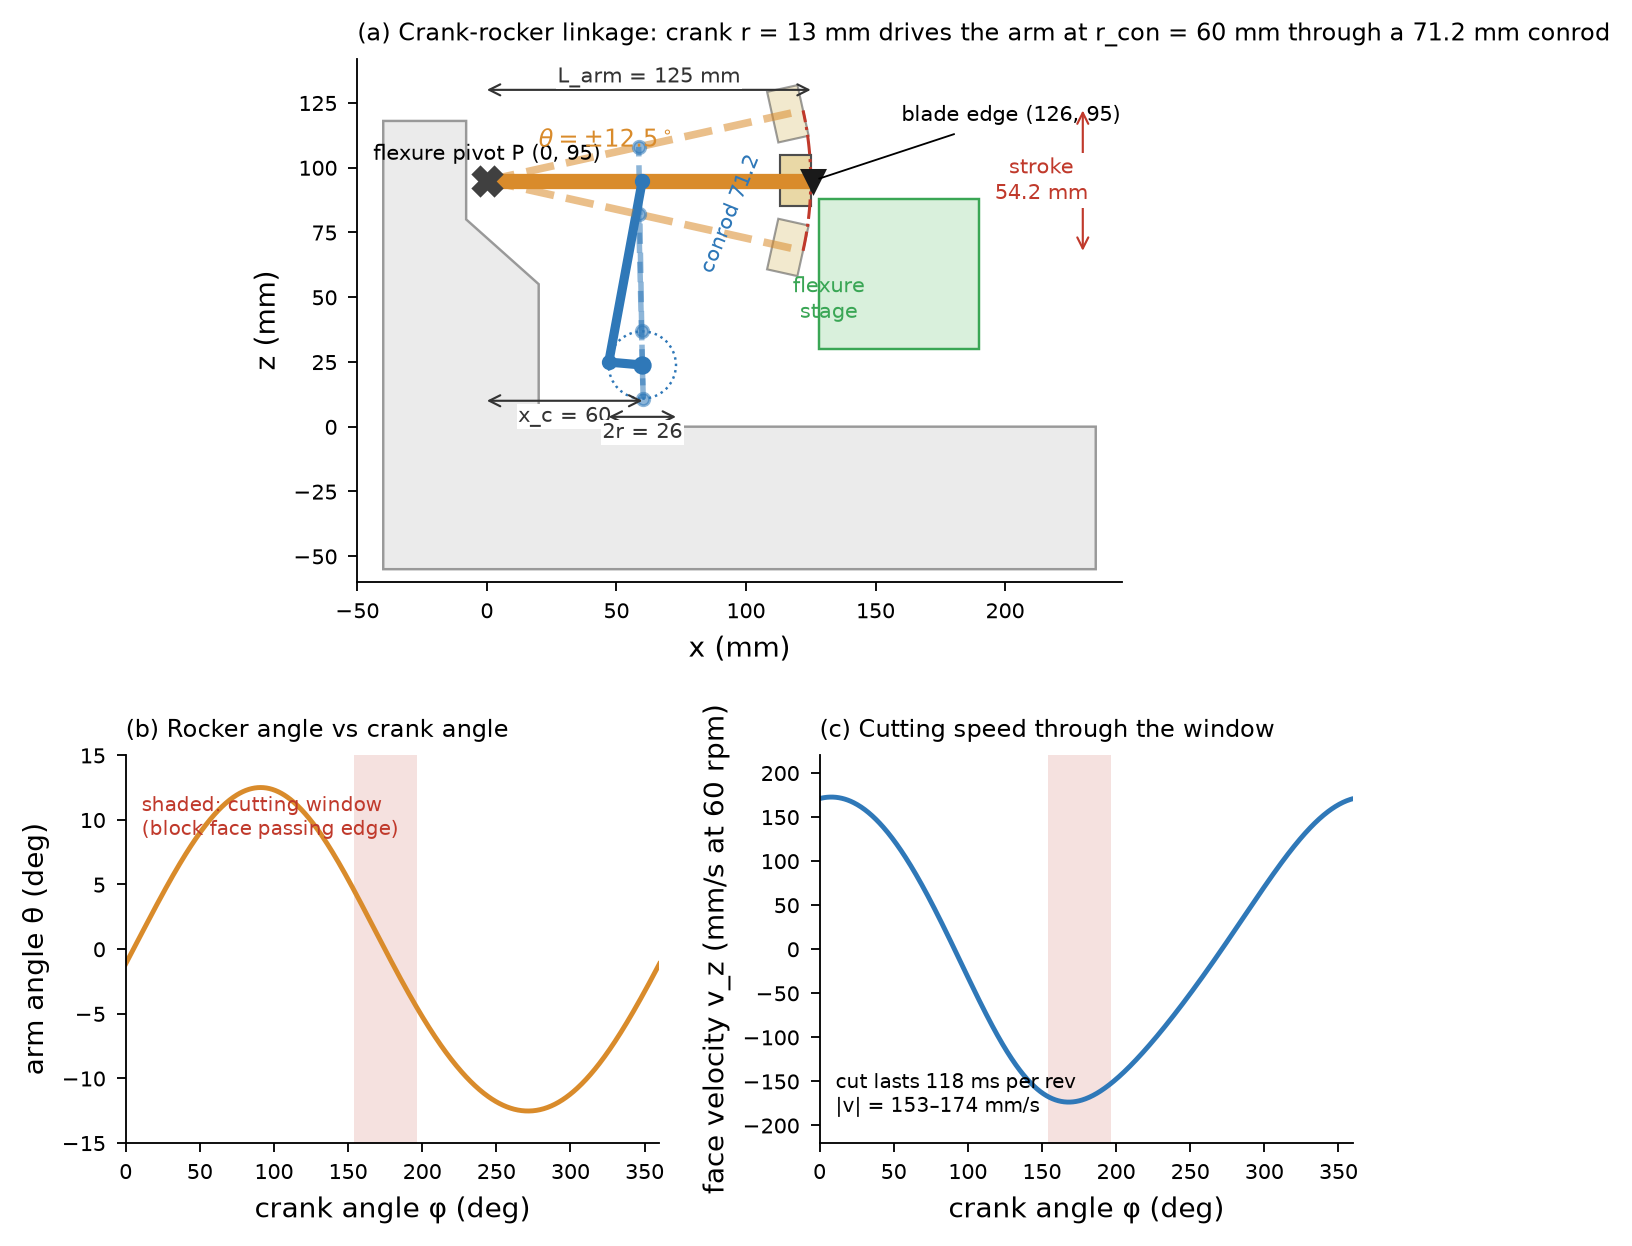
\includegraphics[width=\linewidth]{fig8_mech_kinematics.png}
\caption{Crank-rocker kinematics. (a)~Linkage to scale at mid-stroke (solid) and at the two extremes (dashed), with the block on the arm tip, the face arc (red dash-dot) and the stationary blade edge. (b)~Arm angle $\theta$ against crank angle $\varphi$; the shaded band is the cutting window, during which the \SI{20}{\milli\metre} face passes the edge ($|\theta|<\ang{4.6}$ on the down-stroke). (c)~Vertical face velocity at 60~rpm.}
\label{fig:mkin}
\end{figure}

\FloatBarrier
\subsection{The cut: blade and block geometry}
The blade (6) is a standard disposable low-profile blade ($80\times8\times\SI{0.25}{\milli\metre}$, \ang{35} included facet angle) clamped on the printed holder (7) behind a \SI{1.0}{\milli\metre} steel pressure strip, with the edge \SI{2.5}{\milli\metre} proud of the strip. The holder leans the blade back \ang{27} from the vertical block face. With a \ang{35} wedge the three angles at the edge (Fig.~\ref{fig:mblade}a) are therefore
\begin{equation}
\alpha_{\mathrm{clearance}} = 27^\circ-\tfrac{35^\circ}{2}=\ang{9.5},\qquad
\gamma_{\mathrm{rake}} = 90^\circ-27^\circ-\tfrac{35^\circ}{2}=\ang{45.5},\qquad
\alpha+\tfrac{\beta}{2}+\gamma=90^\circ .
\end{equation}
Because the block rides an arc of radius $L_{\mathrm{arm}}=\SI{125}{\milli\metre}$, the face tangent rotates with $\theta$ during the cut, and the instantaneous clearance sweeps $9.5\pm4.6^\circ$ (4.9--\ang{14.1}) across the face, inside the 3--\ang{15} window practitioners recommend~\citep{Bayley1955,Willis1995}. The same arc means the cut face is cylindrical, with sagitta
\begin{equation}
h=L_{\mathrm{arm}}-\sqrt{L_{\mathrm{arm}}^2-(b/2)^2}=\SI{401}{\micro\metre}\quad(b=\SI{20}{\milli\metre}),
\end{equation}
but since every stroke follows the same arc about the same (flexure-defined) centre, the arc is trimmed into the block once and successive sections (differences between successive arcs) are of uniform thickness (Fig.~\ref{fig:mblade}b). The pressure strip top sits \SI{2.5}{\milli\metre} below the edge along the blade, which places it just outside the block's swept circle; this is the geometric reason the \SI{2.0}{\milli\metre} overhang discussed in Sec.~\ref{sec:levers} is not available.

\begin{figure}[!htbp]\centering
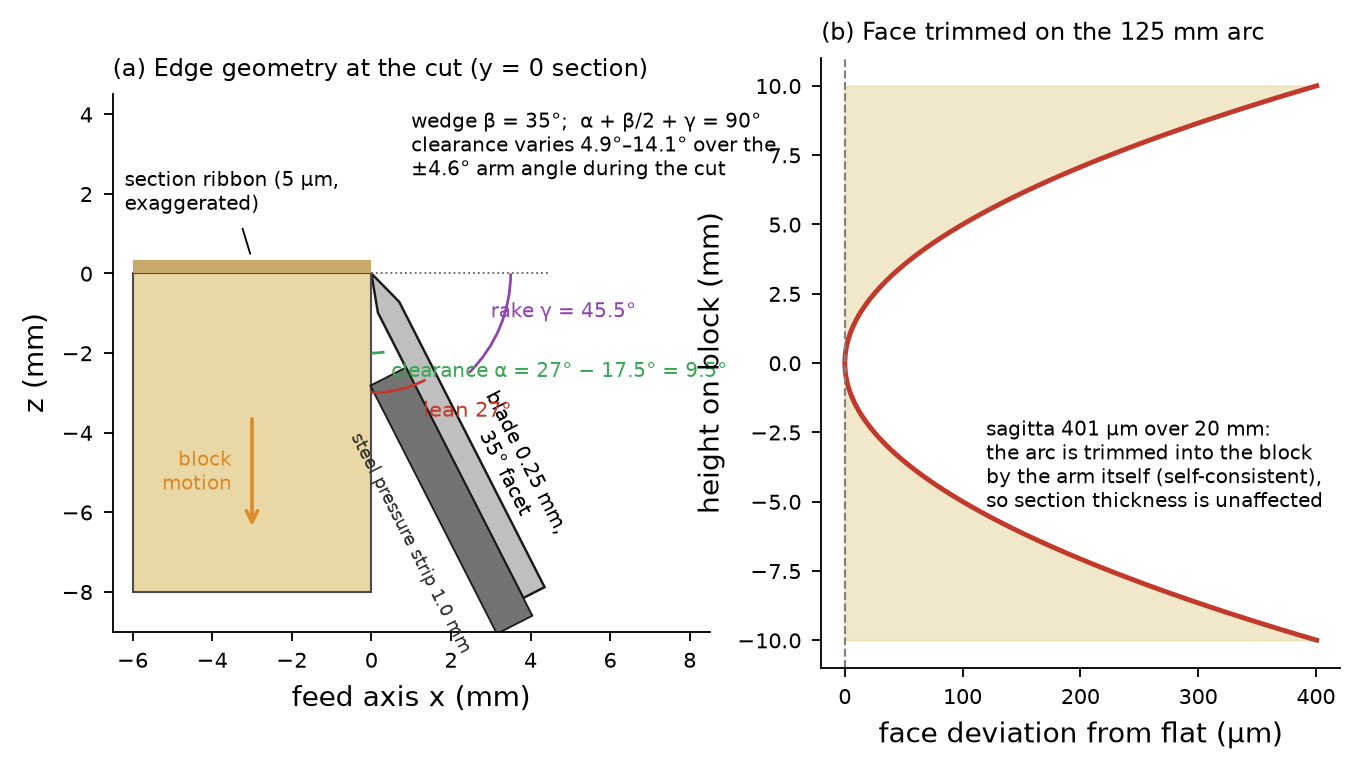
\includegraphics[width=\linewidth]{fig9_mech_blade.png}
\caption{Edge geometry. (a)~Mid-plane section at the cut: block (moving down), blade leaning \ang{27}, steel pressure strip, and the clearance, wedge and rake angles. (b)~Deviation of the arc-trimmed face from a plane over a \SI{20}{\milli\metre} block.}
\label{fig:mblade}
\end{figure}

\FloatBarrier
\subsection{The arm pivot: a cross-strip flexure}
The arm (3) is not on a pin or a bearing. Its root is held to the tower by three strips of \SI{0.20}{\milli\metre} feeler-gauge steel (2), two in one plane (10~mm wide each, at $y=\pm15$\,mm) and one in the perpendicular plane (20~mm wide, at $y=0$), crossing at the pivot axis with \SI{20}{\milli\metre} free length and clamped at both ends under printed pads with M3 screws (Fig.~\ref{fig:mpivot}a). The arm rotates by bending the strips; there is no sliding surface, so there is no backlash, no lubrication and no wear, and the restoring torque is elastic:
\begin{equation}
k_\theta=\sum_i\frac{E\,w_i t^3}{12\,L}=\SI{0.267}{\newton\metre\per\radian},\qquad
\sigma_{\max}=\frac{E\,t\,\theta_{\max}}{2L}=\SI{218}{\mega\pascal},\qquad
T_{\max}=k_\theta\theta_{\max}=\SI{0.058}{\newton\metre}.
\end{equation}
The stress is a factor 2 below the fatigue limit of hardened spring strip and 5 below yield. Along the feed axis the pivot is loaded in tension/compression of the strips and is very stiff (\SI{40}{\newton\per\micro\metre}; \SI{0.025}{\micro\metre\per\newton} in the loop). The price of a cross-strip pivot is a second-order shift of the rotation centre, $\approx0.1\,L\theta^2\approx\SI{95}{\micro\metre}$ at full swing~\citep{Wittrick1948,Haringx1949,SmithChetwynd2017}; because it is a deterministic function of $\theta$ it reshapes the arc slightly but is identical stroke to stroke, so it does not enter the thickness budget. Making the middle strip twice as wide as the outer two and placing it between them balances the two strip planes about $y=0$, so the pivot has no net twist about $z$ when the arm is loaded off-centre.

\FloatBarrier
\subsection{The feed train: differential screw, ratchet drum and selector}
The feed moves the blade, not the specimen. The blade stage (8) is a monolithic parallelogram: a platform on two \SI{1.0}{\milli\metre} PLA plates (front plate \SI{60}{\milli\metre} wide, rear pair $2\times20$\,mm) \SI{44}{\milli\metre} tall, so the platform translates along $x$ with no sliding joint. A tab hanging from the platform carries an M8$\times$1.0 nut; a fixed upstand on the stage foot carries an M8$\times$1.25 nut. One screw assembly (11) threads through both: an M8$\times$1.0 bolt in the tab, a printed coupler with a jam nut, and an M8$\times$1.25 rod in the frame nut, ending in the ratchet drum (12), two jam nuts and the feed knob (14). Turning the screw one revolution advances it \SI{1.25}{\milli\metre} through the frame nut, while the tab nut retreats \SI{1.00}{\milli\metre} along the screw (Fig.~\ref{fig:mscrew}a); the stage therefore moves by the difference,
\begin{equation}
\Delta x_{\mathrm{rev}}=p_1-p_2=1.25-1.00=\SI{0.25}{\milli\metre},\qquad
\Delta x_{\mathrm{tooth}}=\frac{\Delta x_{\mathrm{rev}}}{50}=\SI{5.0}{\micro\metre}.
\end{equation}
The flexure plates preload the tab against the screw (\SI{4.9}{\newton} at full travel), so the stage always rests on one thread flank and lead-screw backlash is removed. Three consequences follow from the differential principle. (i)~\emph{Reduction}: the screw body translates five times farther than the stage, so the \SI{14}{\milli\metre} drum, not a thin wheel, keeps the pawl engaged over the $\pm$\SI{5}{\milli\metre} screw excursion that accompanies the $\pm$\SI{1}{\milli\metre} stage travel (400 sections at \SI{5}{\micro\metre} per reset). (ii)~\emph{Tolerance}: only the \emph{difference} of the two pitches matters, so $\delta t/t=(\delta p_1-\delta p_2)/\SI{0.25}{\milli\metre}$; with 1\,\% independent local pitch errors this contributes \SI{0.37}{\micro\metre} (1~s.d.) at \SI{5}{\micro\metre} (Sec.~\ref{sec:levers}). (iii)~\emph{Resolution without precision parts}: both threads are ordinary rolled hardware; the micrometre-scale motion lives in steel while the printed parts only have to hold nuts.

The thickness selector (13) is a sector shield on the stage column that masks all but $k=1\ldots6$ teeth from the pawl finger, so each stroke advances $5k$\,\si{\micro\metre} (Fig.~\ref{fig:mscrew}b). The coarse approach after loading a new block is independent of the fine feed: the stage foot is clamped to the deck through $\pm$\SI{10}{\milli\metre} slots by two M6 knobs (9) and is pushed against an M6 screw in a side boss (10).

\begin{figure}[!htbp]\centering
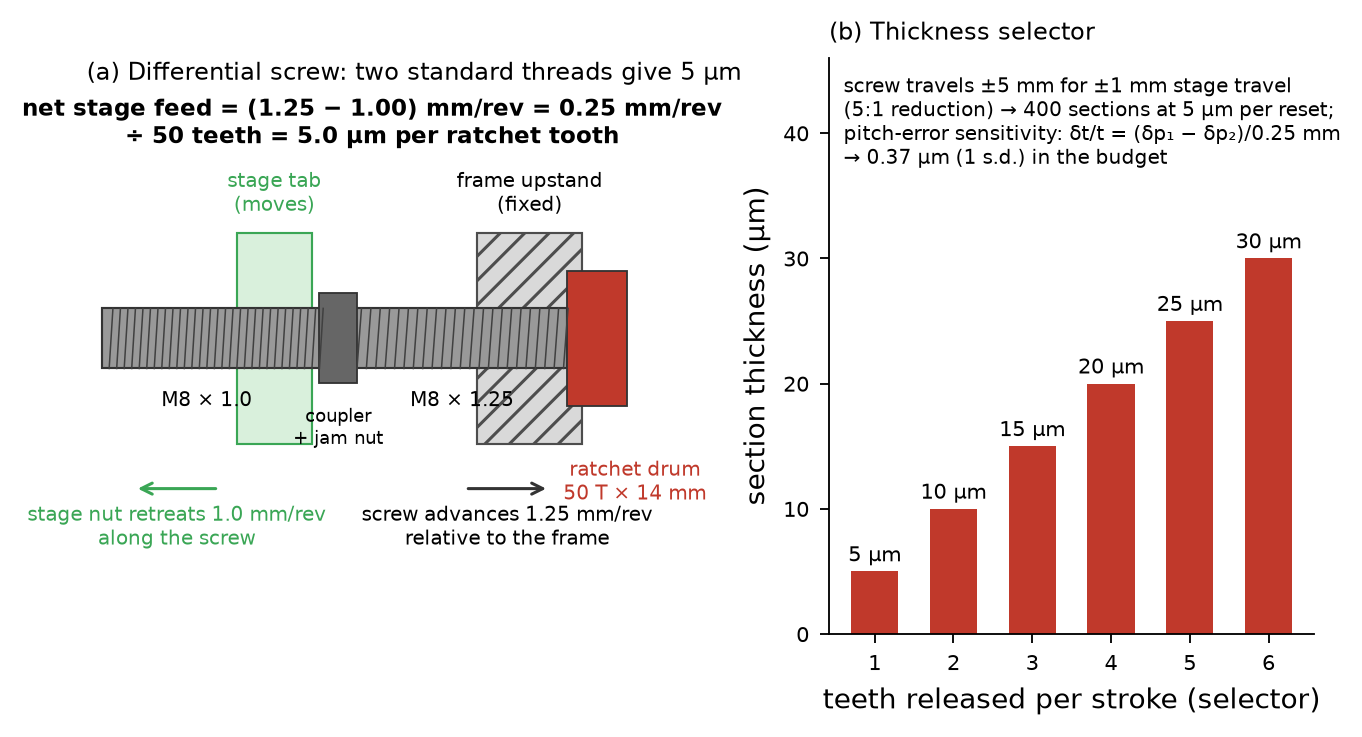
\includegraphics[width=\linewidth]{fig10_mech_screw.png}
\caption{Fine feed. (a)~Differential screw: the frame nut (M8$\times$1.25) and the stage-tab nut (M8$\times$1.0) move the stage by the pitch difference, \SI{0.25}{\milli\metre} per revolution, divided into 50 ratchet teeth. (b)~Selector settings and the resulting nominal section thickness.}
\label{fig:mscrew}
\end{figure}

\FloatBarrier
\subsection{Feed actuation: how one turn makes one section}
A vertical pawl rod (15) slides in a guide on the stage column; its finger rests on the drum teeth under gravity and a light spring. A striker bar (16) fixed to the arm reaches over the rod's flag. On the up-stroke, once the arm passes $\theta\approx\ang{6}$ (block \SI{13}{\milli\metre} clear of the edge) the bar lifts the rod, the finger slides back over the exposed teeth, and at the top of the stroke ($\theta=\ang{12.5}$, lift \SI{22}{\milli\metre}) it has ridden over $k$ teeth. As the arm comes back down past $\theta\approx\ang{6}$ the bar releases the rod; the finger drops behind the $k$th tooth and the rod's weight and spring turn the drum by $k\times\ang{7.2}$, advancing the blade $5k$\,\si{\micro\metre} toward the specimen \emph{before} the face reaches the edge (Fig.~\ref{fig:mtiming}). The feed is therefore complete and the drum is at rest during the cut; the ratchet never moves while the blade is in the block. Return-stroke retraction of the specimen (lifting it off the blade on the up-stroke) is not implemented; the arc geometry gives \SI{3.0}{\milli\metre} of natural retraction at the stroke ends but none at mid-face, so the back of the blade brushes the fresh face on the up-stroke as in the classical Cambridge rocker~\citep{Eaves1954}.

\begin{figure}[!htbp]\centering
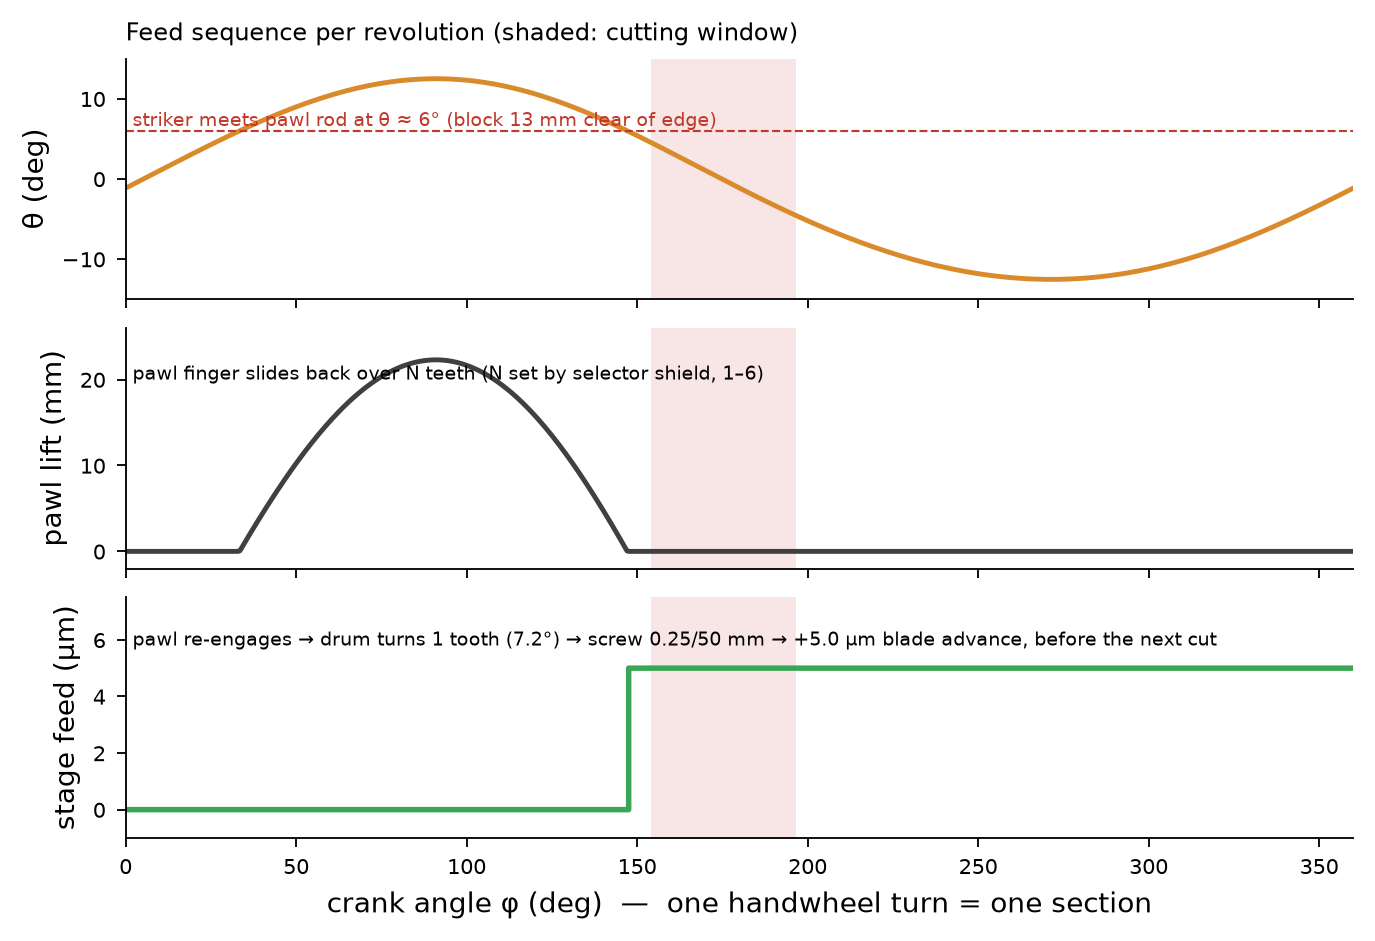
\includegraphics[width=\linewidth]{fig12_mech_timing.png}
\caption{Timing over one handwheel revolution: arm angle, pawl-rod lift and stage feed. The feed step occurs on the down-stroke before the cutting window (shaded).}
\label{fig:mtiming}
\end{figure}

\FloatBarrier
\subsection{The force path and why most of the machine does not matter}
Section thickness is set by the distance between the blade edge and the block face at the moment of the cut. Only parts on the closed path between those two points can change it; everything else (handwheel, crank, rod, drum, pawl) can be as flexible as PLA allows. Walking that loop in the section view (Fig.~\ref{fig:section}): edge~$\rightarrow$ blade overhang~$\rightarrow$ pressure strip and holder~$\rightarrow$ platform~$\rightarrow$ flexure plates (pitching about the nut)~$\rightarrow$ tab nut~$\rightarrow$ screw~$\rightarrow$ frame nut bedded in PLA~$\rightarrow$ upstand, deck, base~$\rightarrow$ tower~$\rightarrow$ strip pivot~$\rightarrow$ arm~$\rightarrow$ cassette clamp~$\rightarrow$ block. The feed-axis compliances add in series (Fig.~\ref{fig:mpivot}b):
\begin{equation}
C_{\mathrm{loop}}=\sum_i C_i=\SI{1.00}{\micro\metre\per\newton},\qquad k_{\mathrm{loop}}=1/C_{\mathrm{loop}}=\SI{1.0}{\newton\per\micro\metre}.
\end{equation}
A steady \SI{2}{\newton} feed-axis cutting force thus opens the loop by \SI{2}{\micro\metre}, but a steady deflection is cut into the block face and does not change the thickness; only its stroke-to-stroke \emph{variation} does (\SI{0.4}{\newton} s.d.~$\rightarrow$ \SI{0.40}{\micro\metre}). The three largest terms are the blade overhang (0.25), the frame between upstand and tower (0.21, FE) and the frame nut bedding in bare PLA (0.20), which is why a pressed brass insert for that nut is the cheapest upgrade (Sec.~\ref{sec:levers}).

\begin{figure}[!htbp]\centering
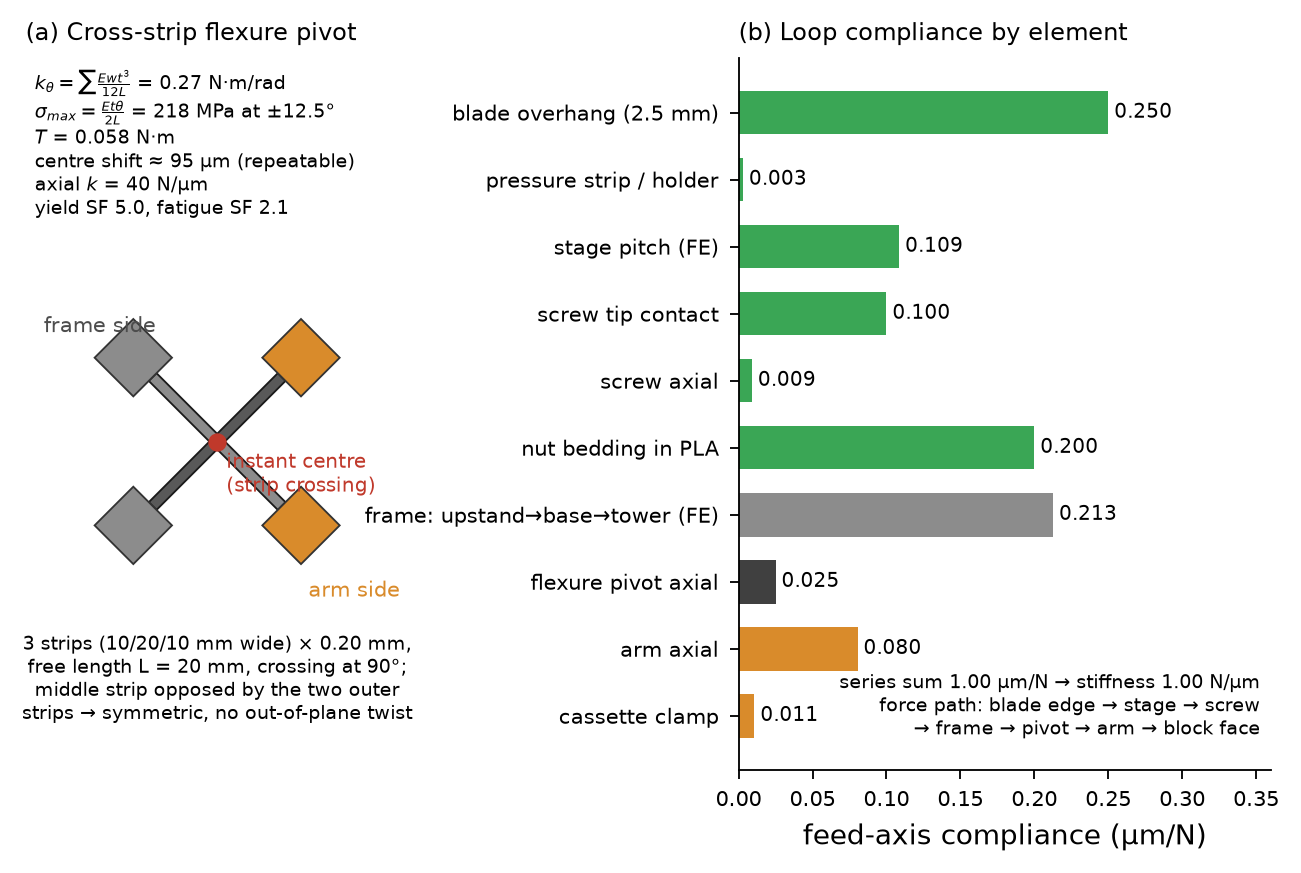
\includegraphics[width=\linewidth]{fig11_mech_pivot_loop.png}
\caption{(a)~Cross-strip pivot geometry and governing relations. (b)~Feed-axis compliance of each element of the metrology loop (green: blade stage group; grey: frame; dark: pivot; orange: arm and clamp).}
\label{fig:mpivot}
\end{figure}

\FloatBarrier
\subsection{Operating sequence}
\begin{enumerate}[nosep,leftmargin=*]
\item Clamp the cassette under the sliding jaw with the M5 thumbscrew (4); the block face must stand proud of the jaw.
\item Loosen the two M6 knobs (9), push the stage toward the block with the coarse screw (10) until the edge is $\sim$\SI{0.5}{\milli\metre} from the face, re-clamp.
\item Set the selector (13) to 6 teeth (\SI{30}{\micro\metre}) and turn the handwheel until the whole face is trimmed to the arc.
\item Set the selector to 1 tooth (\SI{5}{\micro\metre}); each further turn yields one \SI{5}{\micro\metre} section, which the previous section's wax edge carries off as a ribbon.
\item After $\sim$400 sections the stage reaches the end of its $\pm$\SI{1}{\milli\metre} travel: wind the feed knob (14) back 20 turns and repeat step~2.
\end{enumerate}

\FloatBarrier
\subsection{Design revisions driven by the interference audit}
\label{sec:audit}
A boolean interference audit of the assembly (12 crank angles over the full revolution, $\pm$\SI{5}{\milli\metre} screw travel, all part pairs) was re-run after every geometry change. It caught, and the design now reflects: the blade holder entering the specimen's swept circle (fixed by the \ang{27} lean and \SI{2.5}{\milli\metre} overhang); the striker bar passing through the pawl-rod body (bar moved outboard, flag added); the coarse-approach boss fouling the stage foot; the connecting-rod eye placed at the wrong crank position; the screw body translating five times the stage travel (drum ratchet, coupler gap, shield moved from the screw to the column); the connecting rod sweeping through a continuous crankshaft at the bottom of the stroke (built-up two-web crankshaft); and a \SI{1.2}{\milli\metre} offset of the crank centre that made the swing asymmetric ($-\ang{11.4}$ to $+\ang{13.7}$) rather than $\pm\ang{12.5}$ (crank centre lowered to $z=\SI{23.8}{\milli\metre}$). The only residual intersections are intended: pins in bores, strips in clamp pockets, the pawl tooth in the drum (\SI{16}{\milli\metre\cubed}), and the striker bar on the pawl flag between \ang{6} and \ang{12.5} of arm angle, which is the actuation itself.
